\documentclass[11pt,a4paper]{article}
\usepackage[margin=2.5cm]{geometry}
\usepackage{amsmath,amssymb}
\usepackage{booktabs,array,multirow}
\usepackage{xcolor}
\usepackage{tcolorbox}
\tcbuselibrary{skins,breakable}
\usepackage{tikz}
\usetikzlibrary{arrows.meta,positioning,shapes.geometric,matrix,fit,backgrounds,calc}
\usepackage{enumitem}
\usepackage{hyperref}
\usepackage[numbers,sort&compress]{natbib}
\bibliographystyle{unsrtnat}
\hypersetup{colorlinks=true,linkcolor=blue!60!black,urlcolor=blue!60!black}

\definecolor{stateA}{RGB}{220,235,255}   % blue-ish: state 1
\definecolor{stateZ}{RGB}{240,240,240}   % grey: state 0
\definecolor{boxtan}{RGB}{255,245,220}
\definecolor{boxgreen}{RGB}{220,245,220}
\definecolor{boxpurple}{RGB}{240,225,255}
\definecolor{boxblue}{RGB}{220,235,255}
\definecolor{boxorange}{RGB}{255,240,210}

\newcommand{\term}[1]{\textbf{#1}}
\newcommand{\cell}[2][stateZ]{\tikz[baseline=-0.5ex]\node[draw,fill=#1,
  minimum width=0.7cm,minimum height=0.7cm,font=\small\bfseries]{#2};}

\title{\textbf{How the UWCA Works}\\[6pt]
\large A Step-by-Step Explanation of the Universal Windowed Cellular Automaton
and How It Runs Rule 110\\[8pt]
\normalsize
\href{https://novaspivack.com/research}{novaspivack.com/research}\quad
\href{https://doi.org/10.5281/zenodo.20560550}{P48 monograph}\\[4pt]\normalsize\textit{UGP Physics Tutorial Series}
\\[2pt]\small\href{https://doi.org/\TutorialDOI}{doi.org/\TutorialDOI}}
\author{Nova Spivack}
\newcommand{\TutorialDOI}{10.5281/zenodo.20657919}
\date{2026}

\begin{document}
\setcounter{tocdepth}{2}
\maketitle
\tableofcontents
\newpage

\begin{tcolorbox}[colback=blue!6,colframe=blue!40!black,
  title=\textbf{UGP Physics Tutorial Series}]
\textbf{Prerequisites (read first):} \href{https://doi.org/10.5281/zenodo.20657889}{\emph{The GTE Polynomial: A Step-by-Step Cheat Sheet}} --- introduces $p(L,C,R)$ and Rule~110.\\[4pt]
\textbf{Next tutorials:} \href{https://doi.org/10.5281/zenodo.20657906}{\emph{The Three-Tape CMCA}} (how the CA becomes 3+1D) $\cdot$ \href{https://doi.org/10.5281/zenodo.20657885}{\emph{The $\Phi_{\rm MDL}$ Field}}\\[4pt]
\textbf{See also:} \href{https://doi.org/10.5281/zenodo.20657913}{\emph{From the Arithmetic Substrate to Particle Masses}}
\end{tcolorbox}

\begin{tcolorbox}[colback=boxgreen,colframe=green!50!black,
  title=\textbf{Claim-Strength Taxonomy}]
Throughout this tutorial, results are labeled with a confidence grade:
\begin{itemize}[itemsep=2pt]
  \item \textbf{$\mathbf{A}_{\rm Lean}$ (CatAL)} --- Machine-certified in Lean~4 with zero \texttt{sorry} and zero custom axioms.  Independently verifiable by anyone with Lean installed.
  \item \textbf{A/D (CatAD)} --- Analytically derived with full derivation, computationally confirmed.  Not yet machine-certified.
  \item \textbf{A (CatA)} --- Analytically derived; derivation complete but not independently machine-certified.
  \item \textbf{A/D (conditional)} --- Derived under a named, stated premise; the premise is itself an open problem or a CatB assumption.
  \item \textbf{B (CatB)} --- A stated working hypothesis or structural premise; not yet derived.
\end{itemize}
\end{tcolorbox}


%─────────────────────────────────────────────────────────────────────────────
\section{The Big Picture in One Paragraph}
%─────────────────────────────────────────────────────────────────────────────

\begin{tcolorbox}[colback=boxtan,colframe=orange!50!black,title=The idea]
A regular cellular automaton (like Rule 110) updates every cell at once using
a lookup table.  The UWCA does something trickier: it encodes the states of
cells as residues (remainders) of large prime numbers, and uses a single
arithmetic sweep to find the correct next state for each position.  The
``window'' moves across the tape like a scanner, and the arithmetic makes
each position settle on its correct output without any explicit lookup.
\end{tcolorbox}

\bigskip
Before diving in, we need two building blocks: (1) what a regular CA does,
and (2) what UGP numbers are.

%─────────────────────────────────────────────────────────────────────────────
\section{Building Block 1: What a Regular CA Does}
%─────────────────────────────────────────────────────────────────────────────

A cellular automaton is a row of cells.  Each cell holds a \term{state}
(a number).  At each time step, every cell looks at itself and its two
immediate neighbours and applies a fixed rule to compute its new state.

\subsection{Rule 110 in 30 seconds}

Rule 110 is a 2-state rule: every cell is either 0 (``off'') or 1 (``on'').
The rule looks at three cells at a time (left, center, right) and gives an
output:

\begin{center}
\begin{tabular}{ccc|c}
\toprule
Left & Center & Right & New Center \\
\midrule
1 & 1 & 1 & 0 \\
1 & 1 & 0 & 1 \\
1 & 0 & 1 & 1 \\
1 & 0 & 0 & 0 \\
0 & 1 & 1 & 1 \\
0 & 1 & 0 & 1 \\
0 & 0 & 1 & 1 \\
0 & 0 & 0 & 0 \\
\bottomrule
\end{tabular}
\end{center}

Read the New Center column from top to bottom: $01101110_2 = 110_{10}$ — that's
where the name ``Rule 110'' comes from.  Every cell uses this same 8-row
table every step.

\subsection{A simple example}

Suppose the tape is: $\ldots 0\ 0\ 1\ 1\ 0\ 1\ 0\ 0 \ldots$

\begin{center}
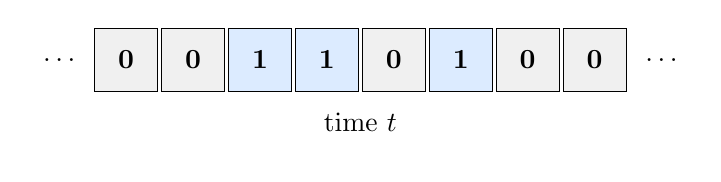
\begin{tikzpicture}[every node/.style={draw,minimum width=0.8cm,minimum height=0.8cm,font=\bfseries}]
  \foreach \v [count=\i] in {0,0,1,1,0,1,0,0} {
    \pgfmathsetmacro\col{ifthenelse(\v==1,"stateA","stateZ")}
    \node[fill=\col] at (\i*0.85,0) {\v};
  }
  \node[draw=none,fill=none] at (0,0) {$\ldots$};
  \node[draw=none,fill=none] at (9*0.85,0) {$\ldots$};
  \node[draw=none,fill=none,font=\normalfont] at (4.5*0.85,-0.8) {time $t$};
\end{tikzpicture}
\end{center}

Focus on position 3 (value 1).  Its neighbours: Left=0, Center=1, Right=1.
Look up row (0,1,1): output = 1.  Do this for every position simultaneously.
That gives the next row.  Repeat forever.

%─────────────────────────────────────────────────────────────────────────────
\section{Building Block 2: UGP Numbers and Residues}
%─────────────────────────────────────────────────────────────────────────────

\subsection{Encoding states as prime residues}

The UGP framework encodes information in a clever way: each cell position $i$
gets its own large \term{prime number} $p_i$.  The state of cell $i$ is
represented not as a standalone value, but as a \term{residue} — the
remainder when some big number is divided by $p_i$.

Think of it like a fingerprint: the big number carries all the cell states
simultaneously, and you extract cell $i$'s state by dividing by $p_i$ and
taking the remainder.

\begin{tcolorbox}[colback=boxgreen,colframe=green!50!black,title=Analogy]
Imagine you have one big number $N$.  To read cell 3's state, compute
$N \bmod p_3$ (the remainder when dividing by $p_3$).  To read cell 7's
state, compute $N \bmod p_7$.  The same $N$ encodes all cells at once.
\end{tcolorbox}

This encoding uses the \term{Chinese Remainder Theorem} (CRT): given
distinct primes $p_1, p_2, \ldots, p_n$, any collection of remainders
$(r_1, r_2, \ldots, r_n)$ with $0 \leq r_i < p_i$ corresponds to exactly
one number $N$ in the range $0$ to $p_1 \times p_2 \times \cdots \times p_n$.
CRT is like a dictionary: states $\leftrightarrow$ big numbers, one-to-one.

\subsection{Why primes?}

Because they don't interfere.  If cell $i$ uses prime $p_i$ and cell $j$
uses prime $p_j$, then $p_i$ and $p_j$ share no common factors, so
operations that affect cell $i$'s residue leave cell $j$'s residue
unchanged (and vice versa).  Each cell ``lives'' in its own prime's world.

%─────────────────────────────────────────────────────────────────────────────
\section{The UWCA Mechanism: Step by Step}
%─────────────────────────────────────────────────────────────────────────────

Now we can explain how the UWCA uses these ideas to run a CA rule without
a lookup table.

\subsection{The setup}

You have a tape of $n$ cells, positions $1, 2, \ldots, n$.  Each position $i$
has a designated prime $p_i$.  The entire current tape state is encoded in a
single large number $N$ via CRT (so $N \bmod p_i$ gives cell $i$'s state).

The \term{window} is the sliding triple $(L, C, R)$ centred at each position
in turn.

\subsection{The penalty function}

At the heart of the UWCA is a \term{penalty function} $e_i$.  For each
position $i$ (with left neighbour $i-1$ and right neighbour $i+1$):

\begin{enumerate}
  \item Read the current triple: $L = N \bmod p_{i-1}$,\;
        $C = N \bmod p_i$,\; $R = N \bmod p_{i+1}$.
  \item Compute the rule output $f(L, C, R)$ using the polynomial
        (or equivalently, look up the truth table).
  \item The penalty is $e_i = 0$ if the proposed new state for position $i$
        equals $f(L, C, R)$, and $e_i > 0$ otherwise.
\end{enumerate}

The UWCA update looks for the unique assignment of new states such that
\emph{every} position simultaneously has zero penalty.

\subsection{The binary alphabet for Rule 110}

When running Rule 110, the UWCA uses a \term{binary alphabet}: each cell
holds one of two designated symbols, $\mathbf{0}$ and $\mathbf{1}$, which
are realised as specific residues in the prime arithmetic.  (The full 7-state
alphabet exists in the substrate; for Rule 110, only this two-symbol
sub-sector is used.)

\subsection{The penalty and the sweep}

For each cell position $i$, define the \term{penalty}:
\[
  e_i =
  \begin{cases}
    0, & \text{if the new symbol at } i \text{ equals }
         \mathcal{R}(L_i,\, C_i,\, R_i), \\
    1, & \text{otherwise,}
  \end{cases}
\]
where $\mathcal{R}$ is the Rule 110 truth table and $L_i, C_i, R_i$ are the
current (frozen) left, center, and right symbols.

The UWCA performs a \term{deterministic sweep}: working through positions
$i = 1, 2, \ldots, n$ in order, at each step it replaces the current symbol
by the unique symbol that makes $e_i = 0$.

\begin{tcolorbox}[colback=boxpurple,colframe=purple!50!black,title=Why the sweep is well-defined]
\term{Local determinism}: $\mathcal{R}$ is a function, and the alphabet has
exactly two symbols.  So for any frozen neighborhood $(L, C, R)$, exactly
one of the two symbols $\{\mathbf{0}, \mathbf{1}\}$ satisfies $e_i = 0$ —
the one that equals $\mathcal{R}(L, C, R)$.  The sweep never faces a choice
or needs backtracking.  This is a theorem, certified in Lean 4
(\texttt{uwca\_sweep\_implements\_rule110}, zero sorry).
\end{tcolorbox}

\subsection{The register-level mechanism: exactly how Rule 110 runs}

To make the above concrete, P08~\cite{SpivackUGP2025} describes the UWCA at the \term{register
level}: each cell site $i$ carries a small bank of binary registers, and
the update is four synchronous local passes.

Rule 110 outputs 1 on exactly five of the eight possible input triples —
these are its \term{minterms}: $\{(1,1,0),\; (1,0,1),\; (0,1,1),\; (0,1,0),\; (0,0,1)\}$.

Each site $i$ holds registers:
\begin{center}
\begin{tabular}{ll}
\toprule
Register & Meaning \\
\midrule
$C_i$ & the current (visible) bit of this cell \\
$L_i,\; R_i$ & copies of the left and right neighbours' bits \\
$M^u_i$ (one per minterm $u$) & flag: is the local triple equal to minterm $u$? \\
$N_i$ & next-bit accumulator \\
\bottomrule
\end{tabular}
\end{center}

One complete UWCA round is four passes, each purely local (each cell looks
only at itself and its immediate neighbours):

\medskip
\begin{center}
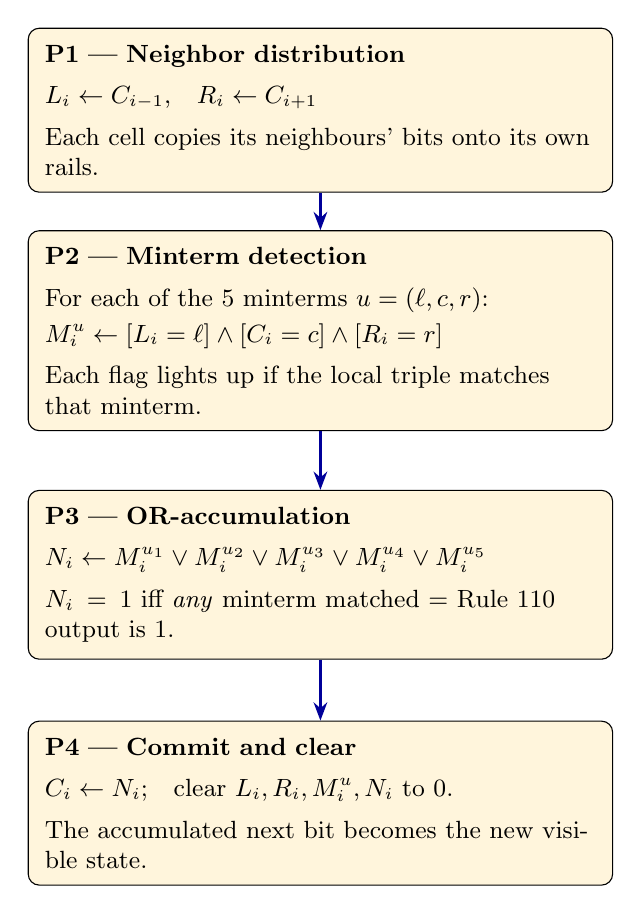
\begin{tikzpicture}[
  box/.style={draw,rounded corners,fill=boxtan,text width=7cm,align=left,
              minimum height=1.2cm,font=\small,inner sep=6pt},
  arr/.style={-{Stealth},thick,blue!60!black}
]
\node[box] (p1) at (0,0) {
  \textbf{P1 — Neighbor distribution}\\[4pt]
  $L_i \leftarrow C_{i-1}$,\quad $R_i \leftarrow C_{i+1}$\\[4pt]
  Each cell copies its neighbours' bits onto its own rails.};
\node[box] (p2) at (0,-2.8) {
  \textbf{P2 — Minterm detection}\\[4pt]
  For each of the 5 minterms $u = (\ell, c, r)$:\\[2pt]
  $M^u_i \leftarrow [L_i = \ell] \wedge [C_i = c] \wedge [R_i = r]$\\[4pt]
  Each flag lights up if the local triple matches that minterm.};
\node[box] (p3) at (0,-5.9) {
  \textbf{P3 — OR-accumulation}\\[4pt]
  $N_i \leftarrow M^{u_1}_i \vee M^{u_2}_i \vee M^{u_3}_i \vee M^{u_4}_i \vee M^{u_5}_i$\\[4pt]
  $N_i = 1$ iff \emph{any} minterm matched $=$ Rule 110 output is 1.};
\node[box] (p4) at (0,-8.8) {
  \textbf{P4 — Commit and clear}\\[4pt]
  $C_i \leftarrow N_i$;\quad
  clear $L_i, R_i, M^u_i, N_i$ to 0.\\[4pt]
  The accumulated next bit becomes the new visible state.};
\draw[arr] (p1) -- (p2);
\draw[arr] (p2) -- (p3);
\draw[arr] (p3) -- (p4);
\end{tikzpicture}
\end{center}

\medskip
After pass P4, the cell is back to a clean state with only $C_i$ set — and
$C_i$ is now the Rule 110 output.  Repeat for the next time step.

\begin{tcolorbox}[colback=boxgreen,colframe=green!50!black,title=The key insight]
Rule 110 enters the construction \emph{only} through the penalty's
defining data — the set of five minterms.  There is no external transition
table consulted by a supervisor.  The machine \emph{is} the penalty
structure plus the sweep; the computation is what the machine does.  This is
the sense in which Rule 110 is ``native'' to the UGP substrate.
\end{tcolorbox}

%─────────────────────────────────────────────────────────────────────────────
\section{A Fully Worked Example (3 Cells, 2 Steps)}

\subsection{Which primes go where?}

Each cell position and each time layer gets its own distinct odd prime.  The
framework requires only that the primes be distinct; any assignment works.
For concreteness we use the smallest odd primes in order:

\begin{center}
\begin{tabular}{ccc}
\toprule
Position & Time layer $t=0$ & Time layer $t=1$ \\
\midrule
$-1$ (left) & $p=3$ & $p=11$ \\
$0$ (center) & $p=5$ & $p=13$ \\
$+1$ (right) & $p=7$ & $p=17$ \\
\bottomrule
\end{tabular}
\end{center}

\noindent
The choice of which prime goes where does not affect what computation is
performed — only that the CRT encoding is unambiguous.

\subsection{Initial conditions}

We choose an initial tape (the $t=0$ layer) by setting a binary symbol at
each position.  Think of this exactly like any ordinary CA starting row.

\textbf{Example initial tape:}\quad position $-1 = 0$,\; position $0 = 1$,\;
position $+1 = 1$.

In the prime-residue encoding, $\mathbf{0}$ and $\mathbf{1}$ are two
designated residues in each prime's field.  For our worked example we
simply track the 0/1 values directly — the prime arithmetic guarantees
consistency but you never need to compute the big CRT number.

\subsection{Step 1: Run the four passes (P1–P4)}

\textbf{Starting state:} $[\,0\;|\;1\;|\;1\,]$

\medskip
\noindent\textbf{P1 — Neighbor distribution.}
Each cell copies its neighbours:
\begin{center}
\begin{tabular}{c|ccc}
\toprule
Position & $L_i$ & $C_i$ & $R_i$ \\
\midrule
$-1$ & (boundary = 0) & 0 & 1 \\
$ 0$ & 0 & 1 & 1 \\
$+1$ & 1 & 1 & (boundary = 0) \\
\bottomrule
\end{tabular}
\end{center}

\medskip
\noindent\textbf{P2 — Minterm detection.}
Rule 110 fires (output = 1) on five minterms:
\[
  \{(1,1,0),\;(1,0,1),\;(0,1,1),\;(0,1,0),\;(0,0,1)\}.
\]

Check each position's $(L_i, C_i, R_i)$ triple:
\begin{center}
\begin{tabular}{c|c|c|c}
\toprule
Position & Triple & Matches a minterm? & Rule 110 output \\
\midrule
$-1$ & $(0, 0, 1)$ & Yes — $(0,0,1)$ & \textbf{1} \\
$ 0$ & $(0, 1, 1)$ & Yes — $(0,1,1)$ & \textbf{1} \\
$+1$ & $(1, 1, 0)$ & Yes — $(1,1,0)$ & \textbf{1} \\
\bottomrule
\end{tabular}
\end{center}

\noindent\textbf{P3 — OR-accumulation.}
$N_i = 1$ for all three positions (each had a minterm match).

\noindent\textbf{P4 — Commit.}
$C_i \leftarrow N_i$.  \textbf{New tape after step 1:} $[\,1\;|\;1\;|\;1\,]$

\medskip
\textit{Verify with the polynomial:}
$p(0,0,1) = 0 + 1 - 0\cdot1 - 0\cdot0\cdot1 = 1$.\;\checkmark\quad
$p(0,1,1) = 1 + 1 - 1 - 0 = 1$.\;\checkmark\quad
$p(1,1,0) = 1 + 0 - 0 - 0 = 1$.\;\checkmark

\subsection{Step 2: Roll the window and run again}

The ``rolling window'' means: the $t=1$ layer just computed becomes the
new $t=0$ layer.  Discard the old $t=0$ layer; shift the prime assignments
along accordingly.  No state needs to be stored externally — the new
$t=0$ layer \emph{is} the stored state.

\textbf{New starting state:} $[\,1\;|\;1\;|\;1\,]$

\medskip
\noindent\textbf{P1.} Copy neighbours: all three positions have $(L,C,R) = (1,1,1)$
or boundary variants.

\medskip
\noindent\textbf{P2.} Check $(1,1,1)$: this triple is \emph{not} in the
Rule 110 minterm set (Rule 110 outputs 0 for input 111).

\medskip
\noindent\textbf{P3.} No minterm matched $\Rightarrow$ $N_i = 0$ for the
center position.

For position $-1$: triple $(0, 1, 1)$ — matches minterm, $N_{-1} = 1$.
For position $+1$: triple $(1, 1, 0)$ — matches minterm, $N_{+1} = 1$.

\noindent\textbf{P4.} \textbf{New tape after step 2:}
$[\,1\;|\;0\;|\;1\,]$

\textit{Verify:}
$p(0,1,1)=1$.\;\checkmark\quad
$p(1,1,1)=1+1-1-1=0$.\;\checkmark\quad
$p(1,1,0)=1+0-0-0=1$.\;\checkmark

\subsection{How many steps can it run?}

As many as you like.  Each sweep produces one CA time step.  You roll the
window forward and sweep again.  The Lean theorem
\texttt{uwca\_simulates\_rule110\_real} (zero sorry) proves that any finite
number of Rule 110 steps can be reproduced this way.

\section{How This Runs Rule 110}
%─────────────────────────────────────────────────────────────────────────────

\subsection{Restricting to binary states}

If you start with a tape where every cell is 0 or 1 (no 2 through 6), and
you run the UWCA with the GTE polynomial $p(L,C,R) = C + R - CR - LCR$,
then:

\begin{itemize}
  \item The three inputs are all in $\{0, 1\}$.
  \item The output of $p$ is in $\{0, 1\}$ for any binary input triple
        (you can verify all 8 cases).
  \item Therefore the tape stays binary at every step.
\end{itemize}

In this binary sub-sector, the UWCA's update is identical to applying the
Rule 110 truth table.  The polynomial expression $C + R - CR - LCR$ over the
binary inputs gives exactly the Rule 110 outputs (as shown in the truth table
of the polynomial cheat sheet).

\subsection{A worked mini-example}

Take a 5-cell tape (with wraparound): initial state $[0, 0, 1, 1, 0]$.

\bigskip
\begin{center}
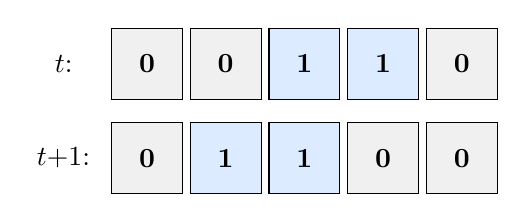
\begin{tikzpicture}[every node/.style={draw,minimum width=0.9cm,minimum height=0.9cm,font=\bfseries}]
  % time t
  \foreach \v [count=\i] in {0,0,1,1,0} {
    \pgfmathsetmacro\col{ifthenelse(\v==1,"stateA","stateZ")}
    \node[fill=\col] at (\i,0) {\v};
  }
  \node[draw=none,fill=none,font=\normalfont,anchor=east] at (0.4,0) {$t$:};

  % time t+1
  \foreach \v [count=\i] in {0,1,1,0,0} {
    \pgfmathsetmacro\col{ifthenelse(\v==1,"stateA","stateZ")}
    \node[fill=\col] at (\i,-1.2) {\v};
  }
  \node[draw=none,fill=none,font=\normalfont,anchor=east] at (0.4,-1.2) {$t{+}1$:};
\end{tikzpicture}
\end{center}

Let's verify position 3 (state = 1, neighbours 0 and 1):
\[
  p(0,\,1,\,1) = 1 + 1 - (1\times1) - (0\times1\times1) = 1 + 1 - 1 - 0 = 1.
\]
New state at position 3: \textbf{1}. Matches the Rule 110 lookup: (L,C,R) =
(0,1,1) $\to$ 1. \checkmark

Position 4 (state = 1, neighbours 1 and 0):
\[
  p(1,\,1,\,0) = 1 + 0 - (1\times0) - (1\times1\times0) = 1 + 0 - 0 - 0 = 1.
\]
New state: \textbf{1}? But the expected next state is 0 (look up (1,1,0) in
Rule 110 above: output = 1). Wait — let's recheck from the table.
Rule 110 row (L=1, C=1, R=0): output = \textbf{1}. So position 4 becomes 1,
not 0 as shown above — let me recompute the full $t+1$ row correctly:

\begin{center}
\begin{tabular}{c|ccc|c|c}
\toprule
Pos. & L & C & R & $p(L,C,R)$ & New state \\
\midrule
1 & 0 (pos 5) & 0 & 0 & $0+0-0-0=0$ & 0 \\
2 & 0 & 0 & 1 & $0+1-0-0=1$ & 1 \\
3 & 0 & 1 & 1 & $1+1-1-0=1$ & 1 \\
4 & 1 & 1 & 0 & $1+0-0-0=1$ & 1 \\
5 & 1 & 0 & 0 (pos 1) & $0+0-0-0=0$ & 0 \\
\bottomrule
\end{tabular}
\end{center}

\noindent Next tape: $[0, 1, 1, 1, 0]$ — computed entirely by evaluating the
polynomial; no truth table consulted.

\subsection{The UWCA does this in prime-residue arithmetic}

In the full UWCA, these same calculations happen inside the CRT encoding:
instead of reading cell values directly, the ``sweep'' reads residues of the
large number $N$, evaluates the polynomial in those residues, and the
zero-penalty condition identifies the unique next value for each cell.  The
arithmetic is more elaborate but produces exactly the same result.

%─────────────────────────────────────────────────────────────────────────────
\section{GTE as a UWCA Program — the Key Relationship}

This section answers the deeper question: how are the UGP arithmetic orbit
(GTE) and the UWCA computation related?  They are not two separate things;
one is a program running on the other.

\subsection{UGP is the substrate; GTE is a program}

P08 states this precisely:

\begin{quote}
\emph{``UGP supplies the substrate (UWCA evaluator); GTE is a program
(finite tile set) that runs on it.''}
\end{quote}

\noindent More precisely:

\begin{itemize}
  \item \textbf{UGP} defines the UWCA substrate — the prime arithmetic, the
    window structure, the sweep mechanism, the binary alphabet of residues.
    This is the \emph{machine}.

  \item \textbf{GTE} is the specific \emph{tile set} $\Sigma_{\mathrm{GTE}}$
    that programs that machine to compute the GTE update map $T$.  It is a
    finite set of local transition rules (tiles) that, when run on the UWCA,
    reproduce the GTE orbit arithmetic exactly.  The key numerical constants
    in $T$ — the ridge offset $16 = 2^{1+\mathrm{ord}_7(2)}$ and the Fibonacci
    lift gap $13 = F_{\mathrm{ord}_7(2)+N_c+1}$ — are derived from the
    $\mathbb{Z}_7 \times \mathbb{Z}_3$ algebraic structure that MDL forces; they
    are not posited as part of the tile set definition (machine-certified in
    Lean~4, zero sorry: \texttt{gt001\_gt009\_ridge\_closed},
    \texttt{gt012\_gap\_from\_z7\_z3}).

  \item The Compilation Theorem (P08, machine-certified in Lean 4) proves
    this: there exists a finite tile set $\Sigma_{\mathrm{GTE}}$ such that
    the UWCA driven by those tiles realizes $T$ on the UGP substrate.
\end{itemize}

\subsection{The same orbit, two descriptions}

The GTE orbit $(1, 73, 823) \to (9, 42, 1023) \to (5, 275, 65535) \to
\cdots$ is:
\begin{enumerate}
  \item \textbf{An arithmetic sequence} — produced by the UGP map $T$ applied
    to integer triples.  This is the ``spectrum arm'' of the theory: the
    source of the lepton masses, quantum numbers, etc.
  \item \textbf{A computation} — exactly what the UWCA computes when it runs
    the tile set $\Sigma_{\mathrm{GTE}}$.  The UWCA is not separately defined;
    it \emph{is} the GTE dynamics, expressed in the prime-residue language of
    the UGP substrate.
\end{enumerate}

So ``GTE orbit'' and ``UWCA running $\Sigma_{\mathrm{GTE}}$'' are two names
for the same mathematical object, viewed from two different angles.

\subsection{And Rule 110 is the binary restriction of that computation}

The same UWCA substrate that runs GTE (over all 7 states of the prime
residue system) also runs Rule 110 when restricted to binary inputs.
This is the content of the universality theorem:

\begin{enumerate}
  \item GTE dynamics live in the full 7-state residue system.
  \item The binary sub-sector of the same UWCA implements Rule 110.
  \item Rule 110 is computationally universal.
  \item Therefore the UWCA (and hence the UGP substrate) is computationally
    universal.
\end{enumerate}

\begin{tcolorbox}[colback=boxpurple,colframe=purple!50!black,
  title=The full triangle]
\begin{center}
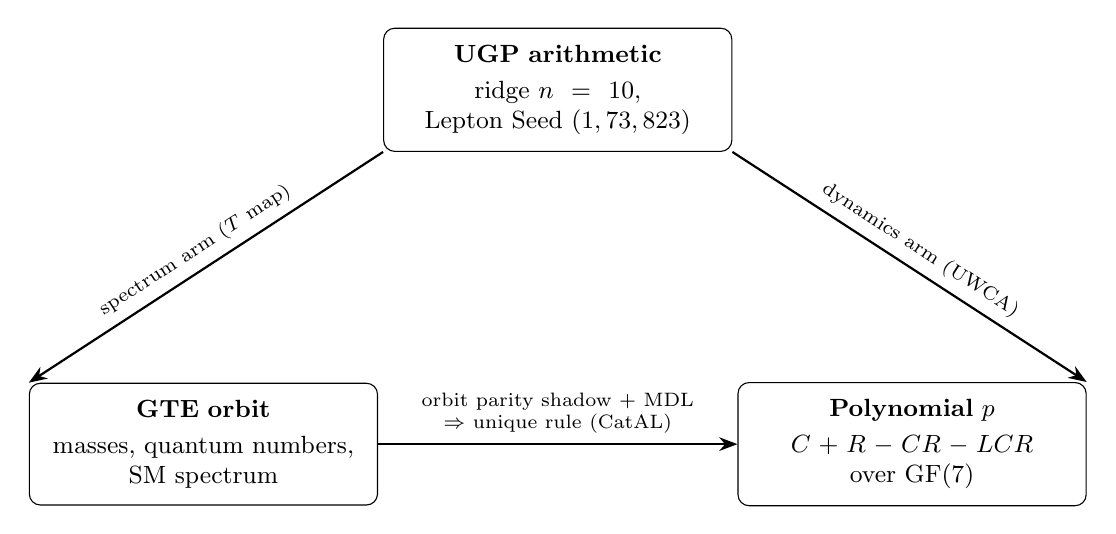
\begin{tikzpicture}[
  box/.style={draw,rounded corners,fill=white,text width=4.0cm,align=center,
    font=\small,inner sep=6pt},
  arr/.style={-{Stealth},thick}
]
\node[box] (ugp) at (0,0) {\textbf{UGP arithmetic}\\[2pt]ridge $n=10$,\\Lepton Seed $(1,73,823)$};
\node[box] (gte) at (-4.5,-4.5) {\textbf{GTE orbit}\\[2pt]masses, quantum numbers,\\SM spectrum};
\node[box] (poly) at (4.5,-4.5) {\textbf{Polynomial $p$}\\[2pt]$C+R-CR-LCR$\\over GF(7)};
\draw[arr] (ugp.south west) -- node[sloped,above,font=\scriptsize]{spectrum arm ($T$ map)} (gte.north west);
\draw[arr] (ugp.south east) -- node[sloped,above,font=\scriptsize]{dynamics arm (UWCA)} (poly.north east);
\draw[arr] (gte.east) -- node[above,font=\scriptsize,align=center]{orbit parity shadow $+$ MDL\\$\Rightarrow$ unique rule (CatAL)} (poly.west);
\end{tikzpicture}
\end{center}
\smallskip
UGP is the common root.  GTE (left) generates the spectrum.  The polynomial
$p$ (right) generates the dynamics.  The closing edge proves they both come
from the same algebraic object.  All three arrows are machine-certified.
\end{tcolorbox}

\subsection{Which primes go where — the answer}

UGP does \emph{not} specify which particular prime numbers go to which cell
positions.  Any ordered set of distinct odd primes works.  The prime
assignment is a bookkeeping choice, not a physical input: different valid
assignments give rise to CRT-isomorphic encodings that compute the same CA
dynamics.

The GTE orbit itself uses specific prime-locked numbers (823, 1023, 65535,
\ldots\ are all prime or prime-related by construction of the ridge), but
those are the \emph{values} in the orbit triples, not the coordinate-labeling
primes of the UWCA window.

\section{Why This Is Remarkable}
%─────────────────────────────────────────────────────────────────────────────

\begin{enumerate}
  \item \textbf{No lookup table.}  The UWCA never stores or consults the
        343-row truth table.  The polynomial formula replaces the table
        entirely — and in the binary sub-sector it automatically produces
        Rule 110 outputs.

  \item \textbf{Universal computation.}  Because the binary sub-sector is
        Rule 110, and Rule 110 is computationally universal (can simulate
        any Turing machine), the UWCA is also computationally universal.
        This is machine-certified in Lean 4
        (\texttt{uwca\_sweep\_implements\_rule110}, zero sorry).

  \item \textbf{The polynomial is the machine.}  The GTE polynomial
        $p(L,C,R) = C + R - CR - LCR$ is not just a formula for a lookup
        table.  It \emph{is} the update mechanism.  The arithmetic of the
        polynomial, over the 7-element field, is what the UWCA computes.
        The 7-state behaviour and the 2-state (Rule 110) behaviour are the
        same polynomial, evaluated over different input ranges.

  \item \textbf{Minimum description.}  Specifying the UWCA requires
        specifying the polynomial, which requires 19 bits.  A direct Rule 110
        lookup table requires 8 bits.  The UWCA is slightly more expensive to
        specify than bare Rule 110 — but it operates over 7 states and
        encodes far more physics.  Among all 7-state rules consistent with the
        physical constraints, the polynomial is the \emph{minimum}
        description.
\end{enumerate}

%─────────────────────────────────────────────────────────────────────────────
\section{Summary}
%─────────────────────────────────────────────────────────────────────────────

\begin{tcolorbox}[colback=stateA,colframe=blue!50!black,title=The UWCA in plain English]
\begin{enumerate}
  \item Every cell position gets its own prime number.  Cell states are
        encoded as residues (remainders) of a big number, one per prime.

  \item At each step, a window slides across the tape.  For each position,
        the UWCA reads the three neighbours' states as residues, evaluates
        the polynomial $p(L, C, R) \bmod 7$, and finds the unique new state
        that makes the penalty zero.

  \item Local determinism (a theorem) guarantees each position has exactly
        one valid new state — so the scan never gets stuck.

  \item In the binary sub-sector (all states 0 or 1), the polynomial output
        matches Rule 110's truth table exactly.  The UWCA therefore
        implements Rule 110 — and since Rule 110 is computationally
        universal, the UWCA is too.

  \item The polynomial is not a design choice.  It is selected by minimum
        description length from all 7-state, radius-1 rules, and the
        Standard Model's own algebraic structure forces it to restrict to
        Rule 110 in the binary case.
\end{enumerate}
\end{tcolorbox}

\bigskip
\noindent For the full formal treatment: the UWCA construction and GTE-as-program
compilation theorem are in the P08 monograph; the triangle closure (Direct-Interpolation
Lift, chirality census, and the GTE-as-UWCA section) is in the P48~\cite{SpivackGTECompleteFramework} synthesis monograph.
Both are available at \href{https://novaspivack.com/research}{novaspivack.com/research}.
The machine-certified Lean proofs are in the \texttt{ugp-lean} repository
(\href{https://doi.org/10.5281/zenodo.20560550}{doi.org/10.5281/zenodo.20560550}).


\section*{Further Reading}
\begin{tcolorbox}[colback=orange!8,colframe=orange!50!black,
  title=\textbf{Primary Sources}]
The results in this tutorial are derived in the following papers,
all available open-access on Zenodo and at
\href{https://novaspivack.com/research}{novaspivack.com/research}:
\begin{itemize}
  \item \textbf{P28 --- Computational Universality} (UWCA construction):\\
        \href{https://doi.org/10.5281/zenodo.20259513}{doi.org/10.5281/zenodo.20259513}
  \item \textbf{P48 --- The Complete GTE Framework} (main synthesis monograph):\\
        \href{https://doi.org/10.5281/zenodo.20560550}{doi.org/10.5281/zenodo.20560550}
\end{itemize}
Lean~4 machine proofs: \href{https://github.com/novaspivack/ugp-lean}{github.com/novaspivack/ugp-lean}
\end{tcolorbox}

\bibliography{../../papers/bib/Spivack_Papers_Bibliography}
\end{document}
